\documentclass[20pt,a4paper]{report}
\usepackage[T2A,T1]{fontenc}
\usepackage[utf8]{inputenc}
\usepackage{blindtext}
\usepackage[russian]{babel}
\usepackage{mwe}
\usepackage{graphbox}
\usepackage[document]{ragged2e}
\usepackage[margin=50pt]{geometry}
\usepackage{longtable}
\usepackage{fontspec}
\usepackage{float}
\usepackage{titlesec}
\usepackage{setspace}
\usepackage{minted}

\usepackage{hyperref}
\hypersetup{
    colorlinks,
    citecolor=black,
    filecolor=black,
    linkcolor=black,
    urlcolor=black
}

\setstretch{1.5}
\graphicspath{{./images/}}
\setmainfont{LiberationSerif}
\setmonofont{Hack}
\titleformat{\chapter}{\normalfont\LARGE\bfseries}{\thechapter}{1em}{}
\titleclass{\chapter}{straight}
\titlespacing{\chapter}{0pt}{0pt}{5pt}[25pt]


\begin{document}
	\begin{titlepage}
		\begin{minipage}{0.3\textwidth}
		
\includegraphics[scale=0.03]{logo.png}	
		\end{minipage}
		\begin{minipage}{0.6\textwidth}\centering
			\textbf{
				Министерство науки и высшего образования Российской Федерации
				Федеральное государственное бюджетное образовательное 
				учреждение высшего образования
				«Московский государственный технический университет
				имени Н.Э. Баумана (национальный исследовательский университет)»
				(МГТУ им. Н.Э. Баумана)
			}	
		\end{minipage}
	
		\vspace{5cm}
		\centering
		\Large
		\textbf{
			Домашнее задание \\
			по курсу «Разработка интернет-приложений» \\
		}

		\vspace{6cm}
		\begin{flushright}
			Выполнил \\ 
			студент группы ИУ5-54Б \\ 
			Сысойкин Е.М. 
		\end{flushright}
		\vspace{5cm}
		Москва, 2020
	\end{titlepage}

	\chapter{Описание задания}
	\large
	\qquad \textbf{Стандартное задание:} \\
	\qquad Создайте прототип веб-приложения с использованием фреймворка Django на основе базы данных, реализующий концепцию master/detail. Прототип должен содержать: \\
		\begin{enumerate}
			\item Две модели, связанные отношением один-ко-многим.
			\item Стандартное средство администрирования Django позволяет редактировать данные моделей. Желательно настроить русификацию ввода и редактирования данных.
			\item Веб-приложение формирует отчет в виде отдельного view/template, отчет выводит HTML-страницу, содержащую связанные данные из двух моделей.
			\item Для верстки шаблонов используется фреймворк Bootstrap, или аналогичный фрейворк по желанию студента.
		\end{enumerate}
	\qquad \textbf{Примечания:} \\
		\begin{enumerate}
			\item Стандартный проект технопарка по Django приравнивается к стандартному варианту ДЗ.
			\item По желанию студента для выполнения ДЗ может быть использован другой фреймворк, аналогичный Django, на любом языке программирования.
		\end{enumerate}
	\qquad \textbf{Расширенные задания, добавляющие +1 балл на экзамене:}
		\begin{enumerate}
			\item Реализация домашнего задания с использованием фреймворка для разработки SPA-приложений (React, Angualar, ...).
			\item Реализация связи много-ко-многим (с возможностью редактирования данных в пользовательском интерфейсе) и развертывание приложения на облачном сервисе (например, heroku).
			\item Реализация в отчете (пункт 3 стандартного задания) графика на основе данных отчета с использованием библиотек JavaScript (например, https://c3js.org/) и развертывание приложения на облачном сервисе (например, heroku).
			\item Подготовка черновика статьи по тематике курса (тематика статьи согласовывается с преподавателем).
		\end{enumerate}
	
	\chapter{Текст программы}
		\qquad \textbf{main.go} \\
		\small
		\inputminted[tabsize=4, linenos, breaklines]{go}{main.go}
		\large	
		
		\qquad \textbf{utils/Databasae.go} \\
		\small
		\inputminted[tabsize=4, linenos, breaklines]{go}{utils/Databasae.go}
		\large	
		
		\qquad \textbf{utils/AppContext.go} \\
		\small
		\inputminted[tabsize=4, linenos, breaklines]{go}{utils/AppContext.go}
		\large	
		
		\qquad \textbf{utils/Gonfigurator.go} \\
		\small
		\inputminted[tabsize=4, linenos, breaklines]{go}{utils/Gonfigurator.go}
		\large	
		
		\qquad \textbf{handlers/Base.go} \\
		\small
		\inputminted[tabsize=4, linenos, breaklines]{go}{handlers/Base.go}
		\large	
		
		\qquad \textbf{handlers/AdminApi.go} \\
		\small
		\inputminted[tabsize=4, linenos, breaklines]{go}{handlers/AdminApi.go}
		\large	
		
		\qquad \textbf{handlers/AdminHandler.go} \\
		\small
		\inputminted[tabsize=4, linenos, breaklines]{go}{handlers/AdminHandler.go}
		\large	
		
		\qquad \textbf{handlers/StockHandler.go} \\
		\small
		\inputminted[tabsize=4, linenos, breaklines]{go}{handlers/StockHandler.go}
		\large	
		
		\qquad \textbf{handlers/DetailHandler.go} \\
		\small
		\inputminted[tabsize=4, linenos, breaklines]{go}{handlers/DetailHandler.go}
		\large	
		
		\qquad \textbf{handlers/MasterHandler.go} \\
		\small
		\inputminted[tabsize=4, linenos, breaklines]{go}{handlers/MasterHandler.go}
		\large	
		
		\qquad \textbf{handlers/SupplierHandler.go} \\
		\small
		\inputminted[tabsize=4, linenos, breaklines]{go}{handlers/SupplierHandler.go}
		\large	
		
		\qquad \textbf{templates/admin.html} \\
		\small
		\inputminted[tabsize=4, linenos, breaklines]{html}{templates/admin.html}
		\large	
		
		\qquad \textbf{templates/error.html} \\
		\small
		\inputminted[tabsize=4, linenos, breaklines]{html}{templates/error.html}
		\large	
		
		\qquad \textbf{templates/stock.html} \\
		\small
		\inputminted[tabsize=4, linenos, breaklines]{html}{templates/stock.html}
		\large	
		
		\qquad \textbf{templates/detail.html} \\
		\small
		\inputminted[tabsize=4, linenos, breaklines]{html}{templates/detail.html}
		\large	
		
		\qquad \textbf{templates/master.html} \\
		\small
		\inputminted[tabsize=4, linenos, breaklines]{html}{templates/master.html}
		\large	
		
		\qquad \textbf{templates/supplier.html} \\
		\small
		\inputminted[tabsize=4, linenos, breaklines]{html}{templates/supplier.html}
		\large	
		
		\qquad \textbf{models/Stock.go} \\
		\small
		\inputminted[tabsize=4, linenos, breaklines]{go}{models/Stock.go}
		\large	
		
		\qquad \textbf{models/Detail.go} \\
		\small
		\inputminted[tabsize=4, linenos, breaklines]{go}{models/Detail.go}
		\large	
		
		\qquad \textbf{models/Supplier.go} \\
		\small
		\inputminted[tabsize=4, linenos, breaklines]{go}{models/Supplier.go}
		\large	
		
		\qquad \textbf{models/DetailStock.go} \\
		\small
		\inputminted[tabsize=4, linenos, breaklines]{go}{models/DetailStock.go}
		\large	
		
	\chapter{Экранные формы}
		\begin{figure}[H]
			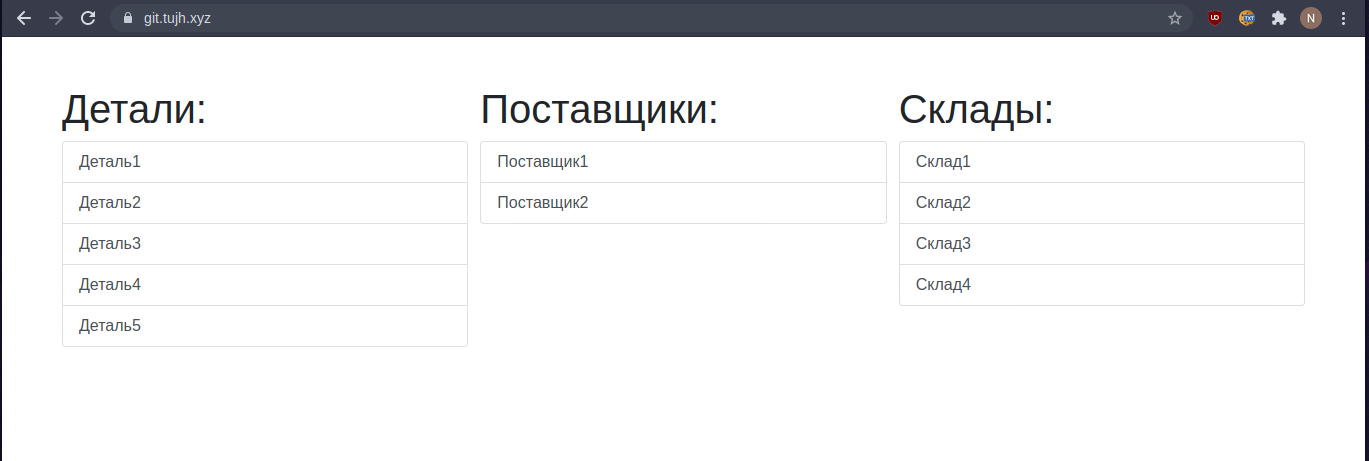
\includegraphics[width=\textwidth]{1.png}
		\end{figure}
		\begin{figure}[H]
			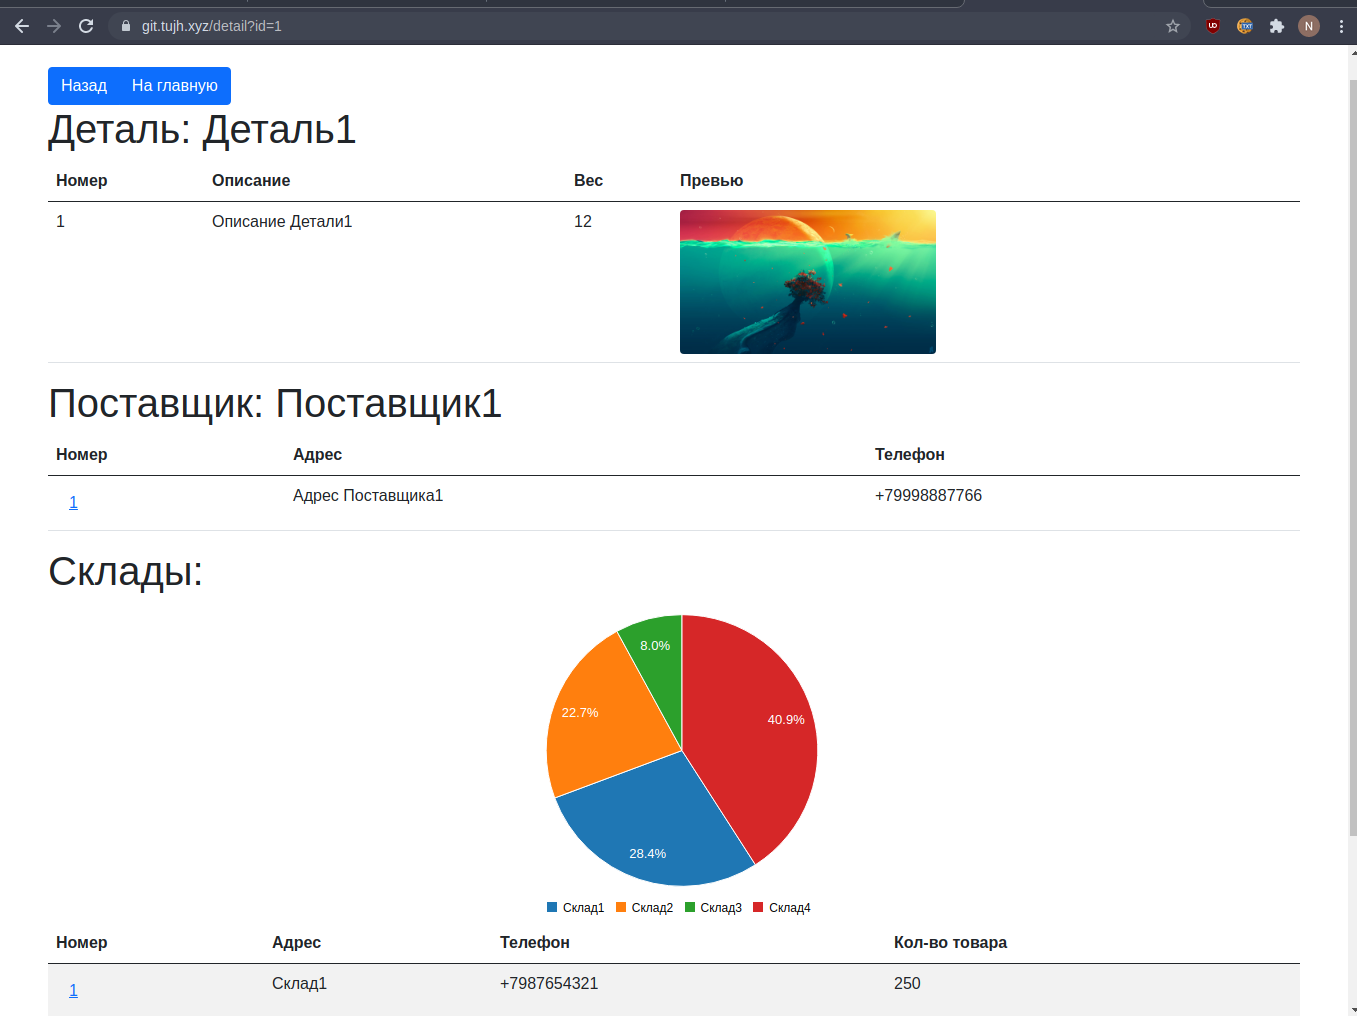
\includegraphics[width=\textwidth]{2.png}
		\end{figure}
		\begin{figure}[H]
			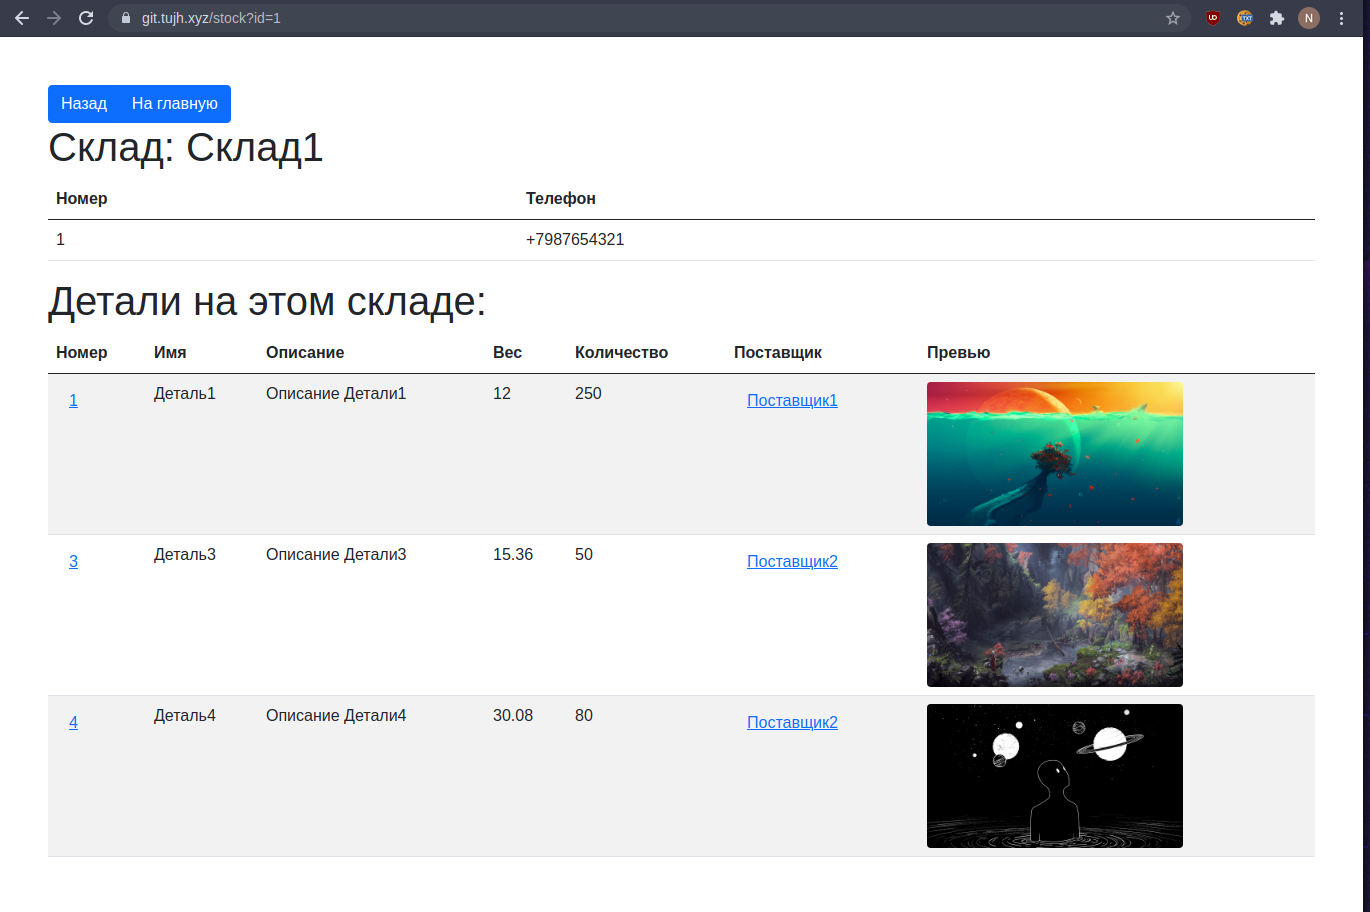
\includegraphics[width=\textwidth]{3.png}
		\end{figure}
		\begin{figure}[H]
			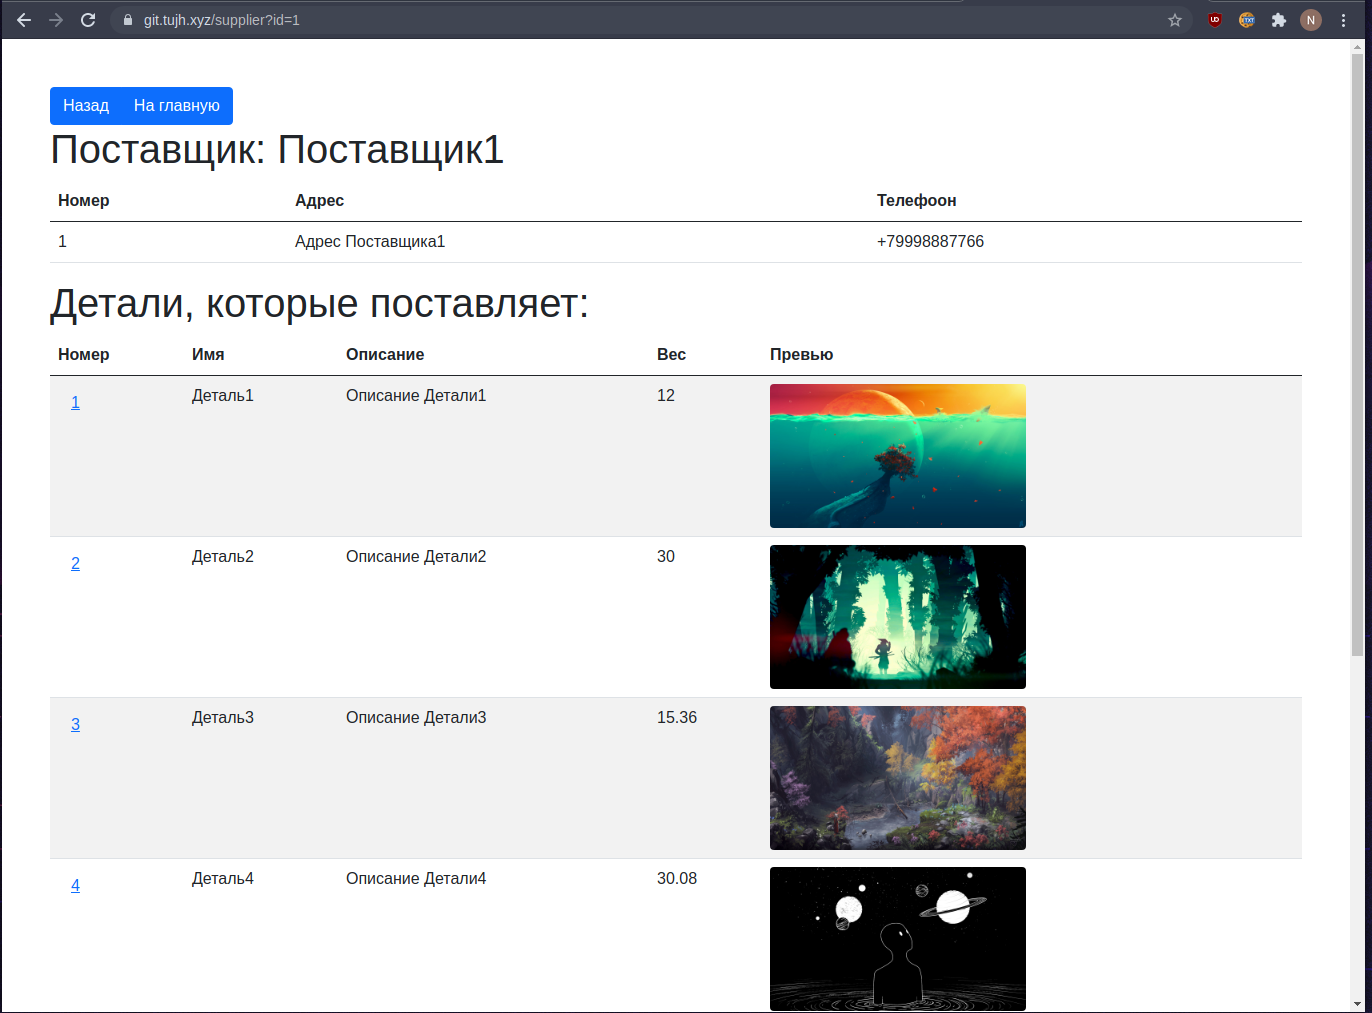
\includegraphics[width=\textwidth]{4.png}
		\end{figure}
		\begin{figure}[H]
			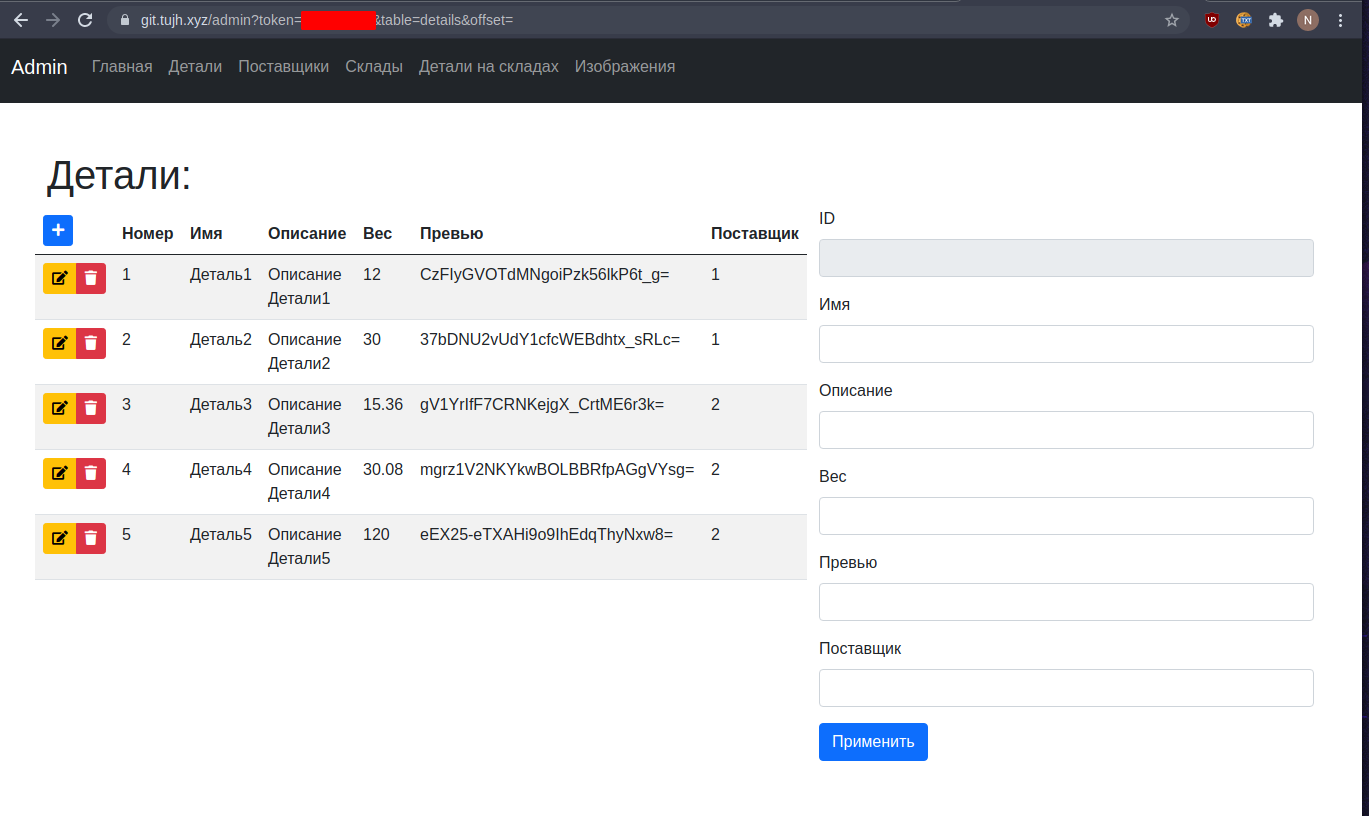
\includegraphics[width=\textwidth]{5.png}
		\end{figure}
		\begin{figure}[H]
			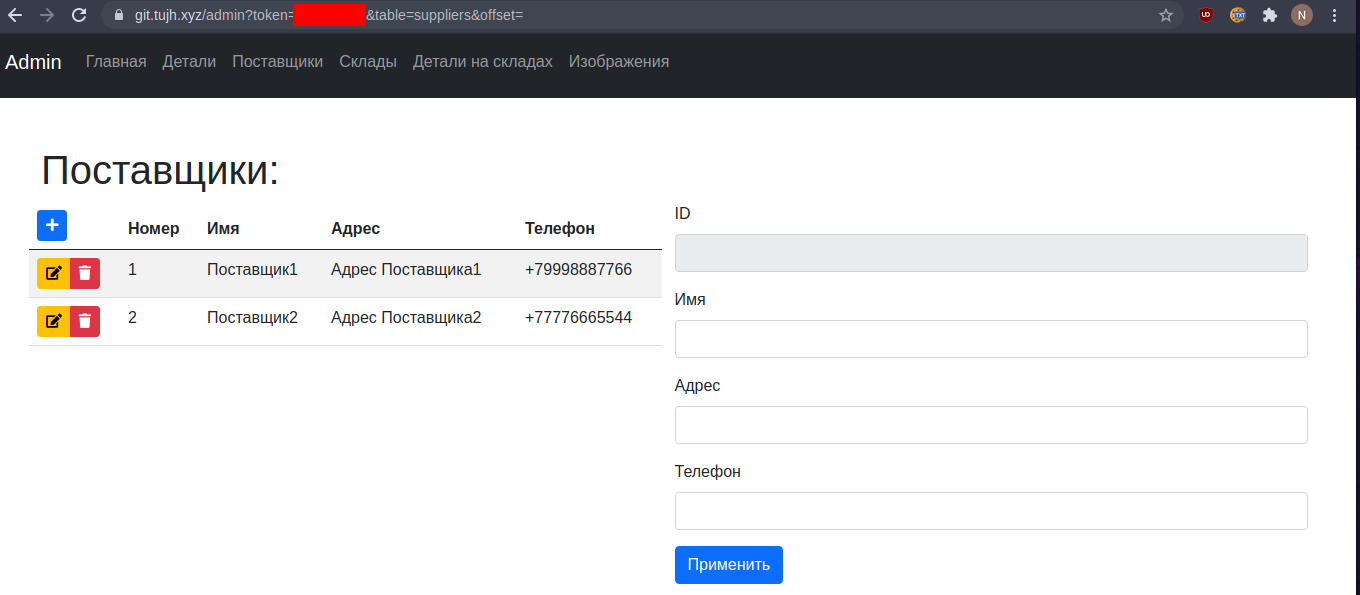
\includegraphics[width=\textwidth]{6.png}
		\end{figure}
		\begin{figure}[H]
			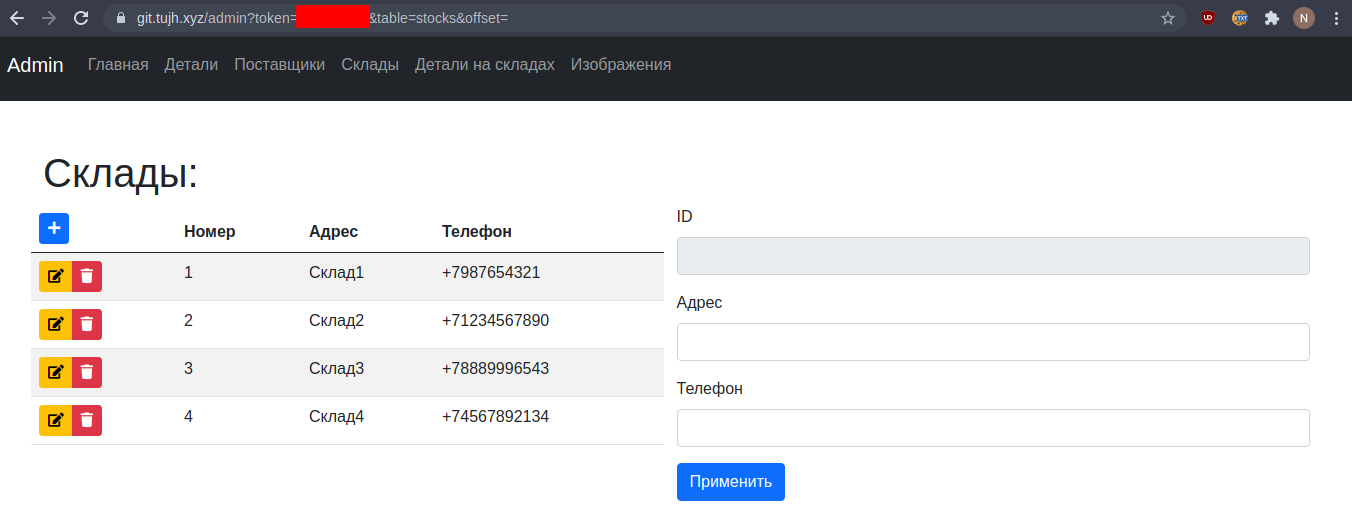
\includegraphics[width=\textwidth]{7.png}
		\end{figure}
		\begin{figure}[H]
			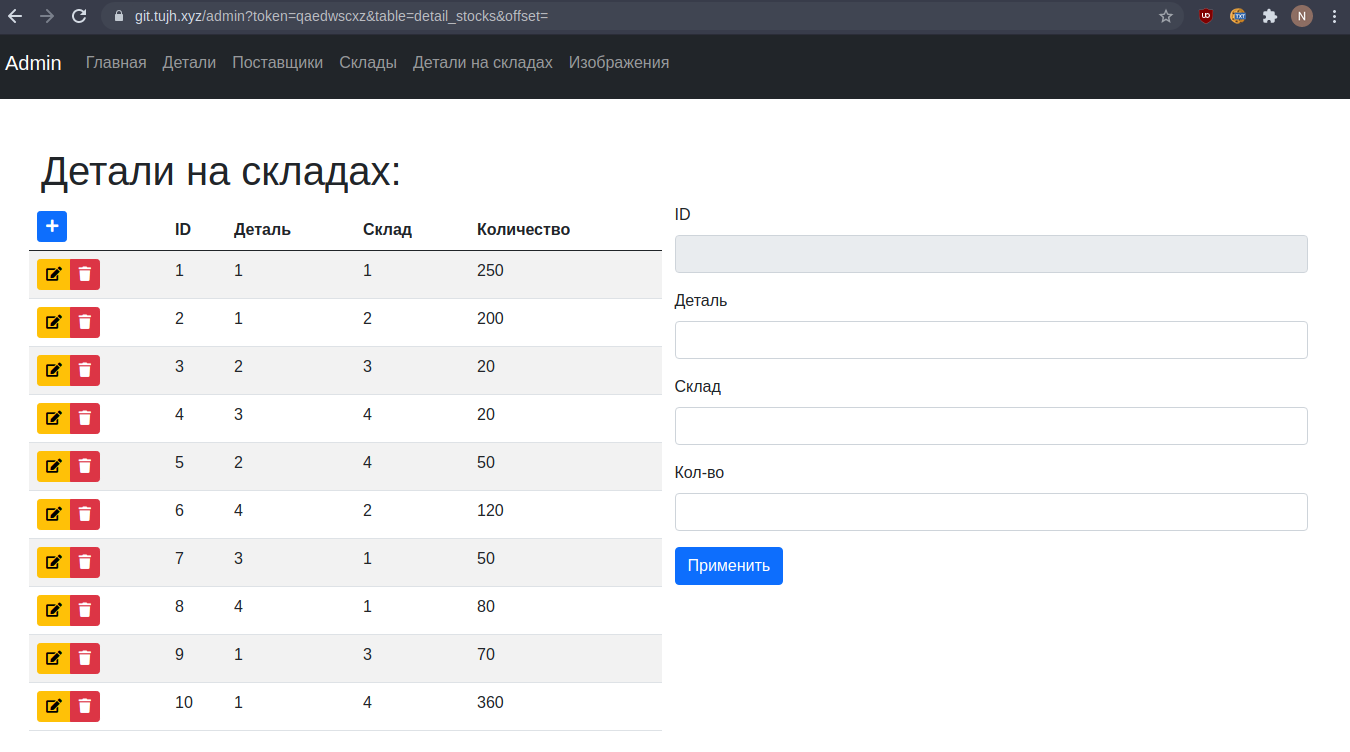
\includegraphics[width=\textwidth]{8.png}
		\end{figure}
		\begin{figure}[H]
			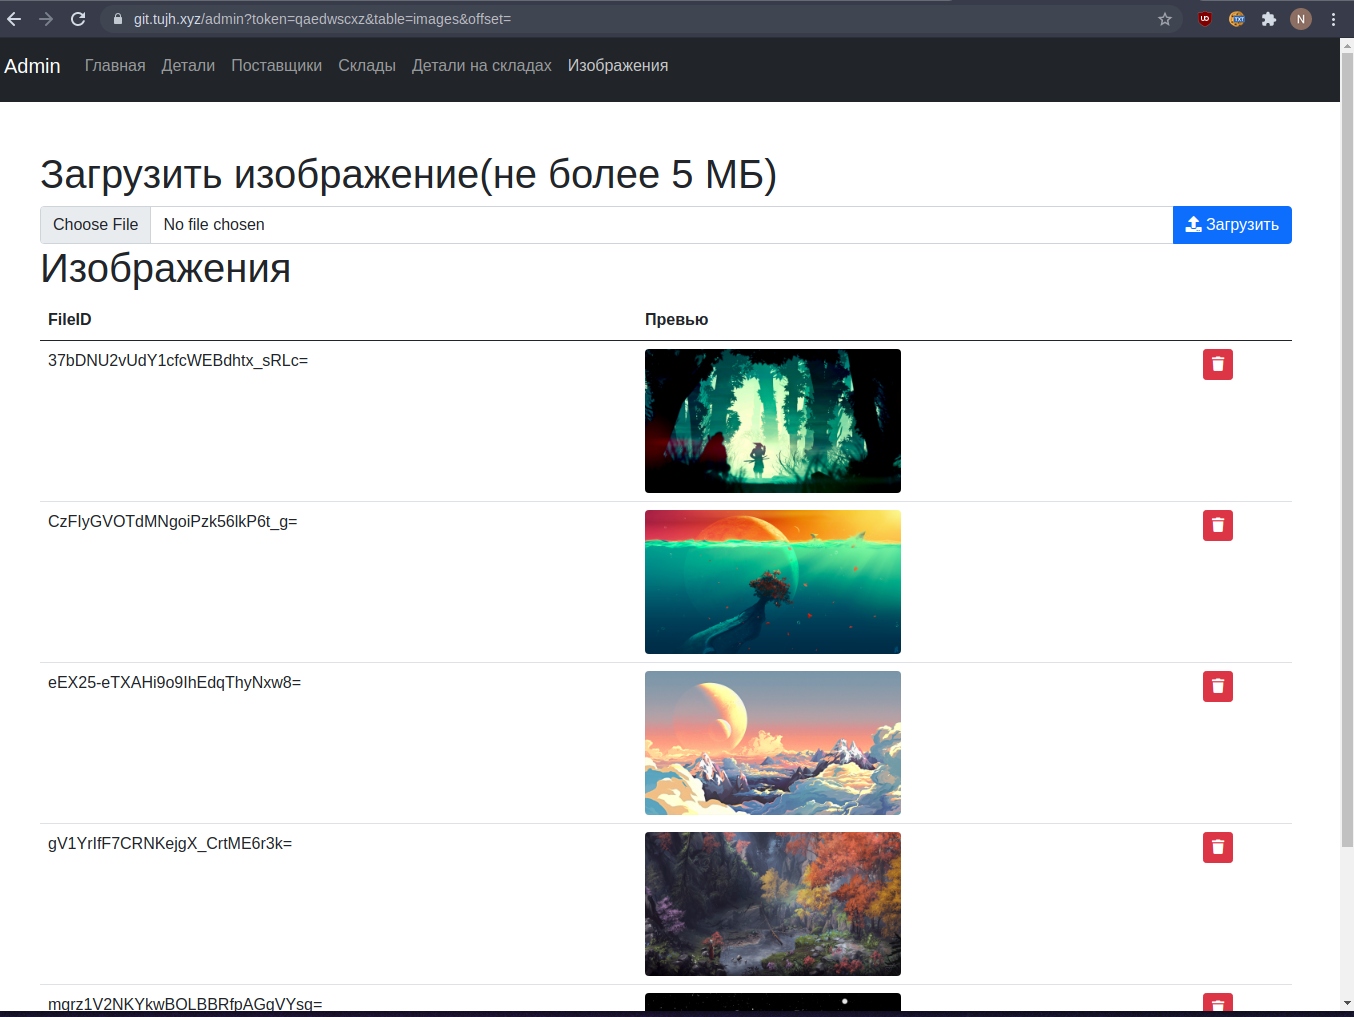
\includegraphics[width=\textwidth]{9.png}
		\end{figure}

\end{document}

